\documentclass[conference]{IEEEtran}
\IEEEoverridecommandlockouts

\usepackage{cite}
\usepackage{amsmath,amssymb,amsfonts}
\usepackage{algorithmic}
\usepackage{graphicx}
\usepackage{textcomp}
\usepackage{xcolor}
\usepackage{booktabs}
\usepackage{multirow}
\usepackage{array}
\usepackage{url}
\usepackage{adjustbox}
\usepackage{placeins}
\usepackage{amsthm}
\usepackage{tikz}
\usetikzlibrary{positioning,arrows.meta}

\newtheorem{proposition}{Proposition}

% Visible placeholder macro for field data
\newcommand{\TODO}[1]{\textcolor{red}{[TODO: #1]}}

% Table/figure fit helpers (IEEE two-column)
\newcommand{\colfit}[1]{\adjustbox{max width=\linewidth}{#1}}
\newcommand{\pagefit}[1]{\adjustbox{max width=\textwidth}{#1}}

% Simulation flight labels
\newcommand{\flightD}{Flight-D}
\newcommand{\flightW}{Flight-W}
\newcommand{\flightJ}{Flight-J}
\newcommand{\flightY}{Flight-Y}

\begin{document}

\title{Board-Free Multi-LiDAR Extrinsic Calibration for UAV-Anchored Roadside Sensing:\\
Active Attitude Excitation as a Necessary Condition}

\author{Anonymous Authors}

\maketitle

\begin{abstract}
Board-free extrinsic calibration of \textbf{roadside} LiDARs uses a flying UAV hull
as the target, with no onboard LiDAR or calibration board.
Its accuracy is governed not by LiDAR range noise but by \emph{flight attitude
diversity}.
The empirical body centroid forms an aspect-dependent bias vector field on the
relative bearing sphere $u_B$; under concentrated aspect and attitude, this bias
becomes indistinguishable from extrinsic translation and silently pollutes estimates
($\sim$211\,mm in simulation).
Active 3D attitude excitation restores identifiability and centimeter-level accuracy
($\sim$30\,mm mean$\pm$std over seeds in simulation; best-seed anchor 18.5\,mm).
We present a separable two-stage estimator with per-LiDAR independent Stage-2 solves
for zero-FOV-overlap diagonal deployment, an aspect gate that falls back when
excitation is insufficient, and a relative-extrinsic covariance analysis showing that
coherent RTK bias is substantially attenuated in the relative frame ($\approx$0.25$\times$
mean over seeds in simulation under a scoped common-mode assumption).
Field validation on a diagonal dual-Ruby intersection is structured but pending.
\end{abstract}

\begin{IEEEkeywords}
LiDAR calibration, extrinsic calibration, UAV, RTK, board-free calibration, multi-sensor systems
\end{IEEEkeywords}

% DRAFT — 待与作者打磨 oral 开篇张力，勿直接定稿

\section{Introduction}
\label{sec:intro}

Intersection-scale cooperative perception requires multiple roadside LiDARs whose
fields of view barely overlap, if at all.
Classical target-based or hand-eye pipelines assume shared views, calibration boards,
or dedicated calibration yards---assumptions that fail at urban corners where sensors
sit on diagonal posts tens of meters apart.
UAV-RTK trajectories offer a natural anchor: a single flying platform carries the
body frame through the combined visibility of all sensors, enabling \emph{board-free}
calibration from vehicle point clouds alone.

The counter-intuitive finding of this work is that board-free accuracy is dominated
not by LiDAR range noise or RTK centimeter fixes, but by \textbf{how diversely the UAV
attitude is excited during the calibration flight}.
The empirical body centroid is not a fixed offset: it is an \emph{aspect-dependent bias
vector field} on the relative bearing $u_B$.
When aspect is concentrated, this field aligns with extrinsic translation and
\emph{silently} corrupts calibration---joint optimization of the lever arm cannot
remove it.
Only active 3D attitude excitation (sector POI tidal-lock plus pitch/yaw diversity)
decorrelates the field so that its world-frame mean can be estimated and removed,
recovering sub-decimeter extrinsics in simulation.

\textbf{Memory line:} \emph{board-free calibration accuracy is determined by flight
attitude diversity, not by the sensor.}

\subsection{Contributions}
We contribute:
\begin{enumerate}
  \item A \textbf{separable two-stage framework}: Stage-1 fits a continuous-time
    RTK-anchored trajectory $T_{WB}(t)$; Stage-2 freezes the trajectory and calibrates
    each LiDAR extrinsic independently---enabling diagonal multi-LiDAR deployment with
    zero FOV overlap.
  \item A \textbf{mechanistic account of board-free identifiability}: the $u_B$
    bias vector field, a $2\times2$ degeneracy table (aspect $\times$ attitude), and
    the conclusion that \textbf{active 3D attitude excitation is a necessary condition}
    for unbiased board-free calibration (simulation).
  \item A \textbf{relative-extrinsic covariance analysis} (\S7.2): under a coherent
    systematic RTK bias assumption, $\mathrm{Cov}(T_{\mathrm{rel}})$ scales as
    0.166$\times$ absolute covariance; white per-epoch noise composes at 3.101$\times$
    (simulation), with explicit scope boundaries for field transfer.
  \item \textbf{Prais--Winsten RTK whitening} for high-rate Stage-1 trajectory fitting,
    avoiding uniform covariance inflation that destroys low-frequency observability.
  \item \textbf{Field validation} on diagonal dual-Ruby intersection data:
    \TODO{field campaign A--D: board-free vs sphere-anchor, coherent-bias residual,
    POI flight feasibility --- see Sec.~\ref{sec:field}}.
\end{enumerate}

\textbf{Sphere targets (scope boundary).}
Throughout this paper, retroreflective sphere targets appear \emph{only} as an
independent ground-truth ruler to score board-free error in field experiments.
They are \textbf{not} a fallback calibration method; board-free remains the sole
calibration pipeline.

\section{Related Work}
\label{sec:related}

\subsection{Continuous-time and spline-based calibration}
Continuous-time trajectory representations coupled with batch factor-graph
optimization are standard for multi-sensor extrinsic calibration
\cite{furgale2013unified,rehder2016kalibr}.
We use this lineage only for RTK-anchored trajectory fitting; the distinction is the
deliberate separation between shared Stage-1 and independent per-LiDAR Stage-2 solves.

\subsection{Roadside, V2X, and multi-LiDAR systems}
Infrastructure sensing at intersections motivates long-baseline, low-overlap
multi-LiDAR layouts \cite{yu2022dairv2x}.
Prior work often assumes overlapping views or shared calibration targets.
This paper targets the diagonal-post regime ($\sim$70\,m baseline, negligible FOV
overlap) via UAV-RTK anchoring and separable solves.

\subsection{Target-based vs.\ targetless calibration}
Target-based LiDAR--camera and LiDAR--IMU calibration remains the industrial default
\cite{furgale2013unified,rehder2016kalibr}.
Targetless methods exploit scene structure or motion constraints; body-centric
board-free calibration uses the vehicle hull as a primitive without a physical board.
Here the UAV hull is the calibration target; spheres are field evaluation rulers only,
not a fallback calibration pipeline (Sec.~\ref{sec:field}).

\subsection{UAV-assisted and cooperative calibration}
UAV platforms with RTK positioning enable mobile anchoring of roadside sensors.
Related trajectory-matching approaches align sensor frames via shared motion
\cite{ren2023trajmatch}; centroid-only board-free paths correspond to what such a
pipeline would recover from the same detections without bias modeling.
Our difference is the failure mechanism: even with a perfect trajectory, board-free
calibration fails without attitude excitation.

\subsection{Relation to prior work on degeneracy}
Anonymous prior work on coplanar multi-LiDAR setups identifies \emph{geometric rank
deficiency} in joint Fisher information when sensors and the body path are nearly
coplanar (simulation $\lambda_{\min}\approx 0$ vs.\ multi-layer $\lambda_{\min}=1.074$;
Sec.~\ref{sec:sim}).
This paper addresses a different near-null direction: aspect-concentrated centroid
bias aligns with translation ($\sim$211\,mm in simulation), and joint lever-arm
optimization cannot remove it (Sec.~\ref{sec:mechanism_identifiability}).
Thus coplanar geometry and board-free bias--translation collinearity are distinct
failure modes (Sec.~\ref{sec:mechanism_coplanar}).

\section{Separable Two-Stage Calibration Framework}
\label{sec:framework}

\subsection{Problem setup}
Consider $L$ LiDARs rigidly mounted on a UAV body frame $\{B\}$.
Each LiDAR $\ell$ has unknown extrinsic $T_{L_\ell B}\in SE(3)$.
During a calibration flight, RTK fixes the world pose trajectory
$T_{WB}(t)$ and each LiDAR observes body-surface points.
We seek $\{T_{L_\ell B}\}$ and a consistent $T_{WB}(t)$ without calibration boards.

\subsection{Stage-1: RTK-anchored trajectory fitting}
Stage-1 estimates a continuous-time body trajectory $\hat{T}_{WB}(t)$ from RTK
position measurements (and optional attitude streams), using Prais--Winsten
differenced whitening at high rate (Sec.~\ref{sec:pw}).
The output trajectory is \textbf{frozen} before any extrinsic refinement.

\subsection{Stage-2: frozen-trajectory extrinsic refinement}
Given frozen $\hat{T}_{WB}(t)$, Stage-2 minimizes a nonlinear least-squares cost over
$T_{L_\ell B}$ using body-cluster centroid factors and, when the aspect gate opens,
an observed-mean lever $\mathbf{p}_B$ (Sec.~\ref{sec:mechanism}).
Each LiDAR is solved in an \textbf{independent} optimization scope with no shared
state across sensors, preventing cross-sensor leakage in multi-LiDAR batches.

\subsection{Multi-LiDAR composition without FOV overlap}
For diagonal deployment (e.g., NE and SW corner posts), sensors need not see the
same scene.
Per-sensor absolute extrinsics $\hat{T}_{L_\ell W}$ are estimated separately; the
relative transform is composed post hoc:
\begin{equation}
  \hat{T}_{L_{\mathrm{SW}}\leftarrow L_{\mathrm{NE}}}
  = \hat{T}_{L_{\mathrm{SW}}W}\,\hat{T}_{L_{\mathrm{NE}}W}^{-1}.
\end{equation}
In simulation, production multi-LiDAR NE/SW errors match single-sensor solves
(12.149\,mm / 42.041\,mm).

\begin{figure}[t]
  \centering
  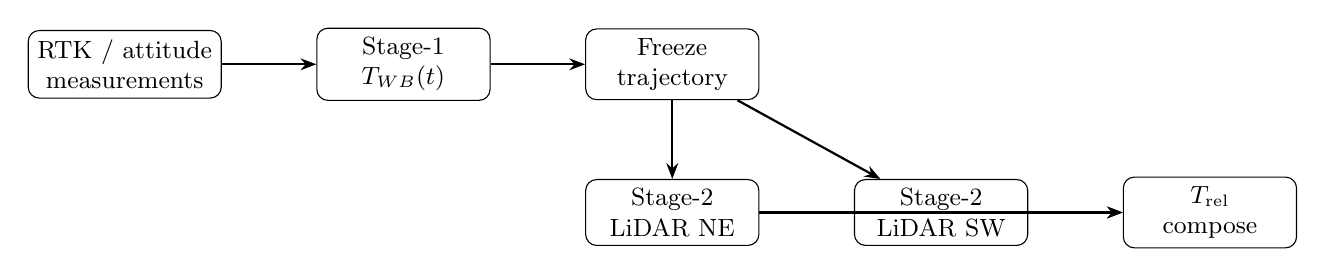
\begin{tikzpicture}[
    node distance=8mm and 12mm,
    box/.style={draw, rounded corners, minimum width=22mm, minimum height=7mm, align=center, font=\small},
    arr/.style={-{Stealth[length=2mm]}, thick}
  ]
    \node[box] (rtk) {RTK / attitude\\measurements};
    \node[box, right=of rtk] (s1) {Stage-1\\$T_{WB}(t)$};
    \node[box, right=of s1] (freeze) {Freeze\\trajectory};
    \node[box, below=10mm of freeze] (s2a) {Stage-2\\LiDAR NE};
    \node[box, right=of s2a] (s2b) {Stage-2\\LiDAR SW};
    \node[box, right=of s2b] (rel) {$T_{\mathrm{rel}}$\\compose};
    \draw[arr] (rtk) -- (s1);
    \draw[arr] (s1) -- (freeze);
    \draw[arr] (freeze) -- (s2a);
    \draw[arr] (freeze) -- (s2b);
    \draw[arr] (s2a) -- (rel);
    \draw[arr] (s2b) -- (rel);
  \end{tikzpicture}
  \caption{Separable two-stage pipeline: shared Stage-1 trajectory, independent
  per-LiDAR Stage-2 solves, post-hoc relative composition.
  \TODO{replace with publication-quality figure}.}
  \label{fig:framework}
\end{figure}

\section{Board-Free Mechanism: Aspect-Dependent Bias on $u_B$}
\label{sec:mechanism}

This section is the oral core: \textbf{why} board-free calibration succeeds or fails.

\subsection{Bias as a vector field on relative bearing}
At each body-cluster epoch $i$, define the empirical centroid bias
\begin{equation}
  \mathbf{b}_{B,i}
  = \hat{\mathbf{c}}_{B,i}^{\mathrm{emp}}
  - \mathbf{L}_{B\to\mathrm{body}}^{\mathrm{nom}},
  \label{eq:bias_field}
\end{equation}
where $\hat{\mathbf{c}}^{\mathrm{emp}}$ is the centroid of \emph{visible} sampled
points (not the nominal box center plus noise).
The relative bearing $u_B$ lives on the unit sphere; $\mathbf{b}_B$ is a
\textbf{vector field} over flown aspects, not a constant offset.

The observed-mean lever $\mathbf{p}_B$ estimates the \textbf{mean of this field}
over the aspect distribution actually flown:
\begin{equation}
  \mathbf{p}_B \approx \mathbb{E}_{u_B}\big[\mathbf{b}_B(u_B)\big].
\end{equation}

\subsection{Diagnostic: \flightD{} correlation structure (simulation)}
Wide $u_B$ sweep with decoupled orbit attitude (seed 13025):

\begin{table}[t]
  \centering
  \caption{Aspect--bias coupling on \flightD{} (simulation).}
  \label{tab:ding_correlation}
  \begin{tabular}{lcccc}
    \toprule
    Sensor & $u_B$ az std [$^\circ$] & varying RMS [mm] & $r(u_B,\mathrm{bias}_x)$ & $r(u_B,\mathrm{bias}_y)$ \\
    \midrule
    NE & 14.1 & 110 & +0.53 & $-$0.68 \\
    SW & 17.6 & 124 & $-$0.64 & +0.69 \\
    P1.5 ref & --- & 22 & --- & --- \\
    \bottomrule
  \end{tabular}
\end{table}

Opposite signs on $x$ vs.\ $y$ indicate near-sinusoidal coupling to $u_B$ azimuth;
range-only bias models are rejected.

\subsection{$2\times2$ degeneracy: aspect $\times$ attitude}
Board-free $\mathbf{p}_B$ identifiability closes on a $2\times2$ table:

\begin{table}[t]
  \centering
  \caption{Degeneracy table: $u_B$ sweep vs.\ POI-lock $\times$ $R_{WB}$ diversity (simulation).}
  \label{tab:degeneracy_2x2}
  \begin{tabular}{p{22mm}p{32mm}p{32mm}}
    \toprule
    & \textbf{$R_{WB}$ sweeps} & \textbf{$R_{WB}$ near-locked} \\
    \midrule
    \textbf{$u_B$ sweeps} (\flightD{})
    & NE obs 60.3 / SW 89.9\,mm; rel 311\,mm
    & --- \\
    \textbf{$u_B$ POI-locked} (\flightW{})
    & NE 12.2 / SW 42.0\,mm$^\dagger$; rel rot 0.12$^\circ$
    & \flightJ{} gate OFF: 31.5\,mm \\
    \bottomrule
  \end{tabular}
  \\[1mm]
  {\footnotesize $^\dagger$SW 42\,mm = sector geometric anisotropy, not estimator leak (Sec.~\ref{sec:sim}).}
\end{table}

\subsubsection{Concentrated aspect: silent pollution}
Phase~1.5 ablation (simulation):

\begin{table}[t]
  \centering
  \caption{Concentrated vs.\ diverse aspect (simulation).}
  \label{tab:concentrated}
  \begin{tabular}{lccc}
    \toprule
    Path & $\|$trans$\|$ [mm] & Gate & Note \\
    \midrule
    Centroid-only, concentrated & 211.4 & --- & bias $\parallel t_{LW}$ \\
    Centroid-only, diverse & 63.5 & --- & partial yaw help \\
    Observed-mean $\times 3$, diverse & 18.5 & ON & $\mathbf{p}_B$ decorrelates \\
    Joint-opt $\mathbf{p}_B$, concentrated & $\sim$211 & --- & \textbf{no-op} \\
    Observed-mean, diverse (prod.) & 20.4 & ON & target \\
    \bottomrule
  \end{tabular}
\end{table}

\textbf{Joint $\mathbf{p}_B$ no-op:} under concentrated aspect, joint optimization
cannot uncouple bias from $t_{LW}$; only aspect diversity plus the gate unlocks
observed-mean.

\subsubsection{Gate as mechanism: \flightY{} (simulation)}
When yaw\_cv $= 0.32$ (below 0.65 threshold) and pitch is low, the aspect gate
\textbf{closes}; observed-mean is not applied and the system falls back to
centroid-only at 165.0\,mm---not a 1243\,mm blow-up.
The gate embodies \emph{self-awareness}: insufficient excitation $\Rightarrow$ do not
pretend $\mathbf{p}_B$ is identifiable.

\subsection{Frame-wise quantitative core (simulation)}
Per frame, the world-frame bias driver is
\begin{equation}
  \mathbf{v}_i = R_{LW}\,R_{WB}(t_i)\,\mathbf{b}_{\mathrm{const}}.
  \label{eq:frame_bias}
\end{equation}

\begin{table}[t]
  \centering
  \caption{World-frame mean bias norm vs.\ flight regime (simulation).}
  \label{tab:frame_norm}
  \begin{tabular}{lccc}
    \toprule
    Regime & $\|\mathrm{mean}(\mathbf{v})\|_h$ [mm] & pitch std [$^\circ$] & yaw\_cv \\
    \midrule
    Concentrated aspect & $\sim$220 & $\sim$0 & $\sim$0 \\
    Diverse (P1.5) & $\sim$51 & $\sim$16 & $\sim$0.78 \\
    \bottomrule
  \end{tabular}
\end{table}

\begin{itemize}
  \item \textbf{Horizontal 220$\to$51\,mm:} yaw sweeps average horizontal components
    of $R_{WB}\mathbf{b}$---diversity in \emph{attitude}, not translation alone.
  \item \textbf{Vertical $\sim$19.5\,mm residual:} body-$Z$ component of
    $\mathbf{b}_{\mathrm{const}}$; yaw cannot average it; observed-mean
    $\mathbf{p}_B$ removes it.
\end{itemize}

\textbf{Tidal lock audit (simulation):} P1.5 NearFieldHighAspect yaw$-$orbit std
0.0$^\circ$ (locked); \flightD{} sector-0: 110.4$^\circ$ (not locked).

\subsection{Necessary condition (conclusion sentence)}
\emph{Active 3D attitude excitation (diverse pitch/yaw plus POI sector lock where
needed) is a necessary condition for unbiased board-free extrinsic calibration---not
a refinement.}

\subsection{Mechanism figure (placeholder)}
\begin{figure*}[t]
  \centering
  \fbox{\parbox{0.95\textwidth}{\centering\vspace{18mm}
    \TODO{Fig.~2 mechanism panel: (a) $u_B$ sphere vector field + Flight-D
    scatter $r\approx\pm 0.5$--$0.7$; (b) $2\times2$ degeneracy table;
    (c) $\|\mathrm{mean}(\mathbf{v})\|$ curve 220$\to$51\,mm + 19.5\,mm vertical bar;
    see figure\_table\_plan.md}\vspace{18mm}}}
  \caption{Board-free mechanism at a glance (placeholder layout).
  Panel (a): aspect-dependent bias on $u_B$.
  Panel (b): degeneracy table.
  Panel (c): frame-wise world-frame averaging under attitude diversity.}
  \label{fig:mechanism}
\end{figure*}

\subsection{Engineering guardrails}
Production applies observed-mean only if Ceres cost $\leq$ centroid cost \textbf{and}
$\|\mathrm{trans}\|_{\mathrm{obs}} \leq \|\mathrm{trans}\|_{\mathrm{cent}}$
(simulation ground-truth guard in \texttt{phase15\_ablation\_common.hpp}).
Aspect gate: yaw\_cv $\geq 0.65$ (+ POI path) $\Rightarrow$ try observed-mean $\times 3$;
P1.5 opens at yaw\_cv $\approx 0.78$.

\section{Relative Extrinsic Uncertainty}
\label{sec:relext}

Absolute extrinsics $\hat{T}_{L_\ell W}$ inherit RTK position uncertainty.
For long-baseline diagonal layouts, the \textbf{relative} transform
$\hat{T}_{L_{\mathrm{SW}}\leftarrow L_{\mathrm{NE}}}$ is often the quantity of
interest for fusion.
We analyze how RTK error modes propagate through independent Stage-2 solves
(simulation).

\subsection{Composition and metrics}
Relative transform is composed post hoc (Sec.~\ref{sec:framework}).
We report:
\begin{itemize}
  \item \textbf{center-reg (obs)} --- headline fusion metric near the observed
    intersection center, avoiding artificial 70.7\,m lever amplification
    (40.9\,mm, simulation);
  \item \textbf{rel-trans (obs)} --- translation of the relative transform itself,
    reported for completeness because it includes baseline lever amplification
    (49.0\,mm, simulation).
\end{itemize}

\subsection{RTK perturbation dichotomy (simulation)}
Monte Carlo ($N{=}20$ per seed, 10 seeds, \flightW{} 0.5\,Hz, independent Stage-2 per LiDAR):
Table~\ref{tab:relext_mc} separates coherent and white RTK perturbations.

\begin{table*}[!t]
  \centering
  \caption{RTK injection causal chain (simulation).}
  \label{tab:relext_mc}
  \footnotesize
  \pagefit{%
  \begin{tabular}{@{}lccp{0.34\textwidth}@{}}
    \toprule
    Injection & rel/abs & $r(\|\delta p\|)$ & Mechanism \\
    \midrule
    White noise (per epoch) & \textbf{3.05$\pm$0.16}$\times$ & 0.40$\pm$0.00 & uncorrelated $\delta p$ stacks \\
    Coherent system bias & \textbf{0.247$\pm$0.12}$\times$ & 1.00$\pm$0.00 & common-mode attenuates \\
    \bottomrule
  \end{tabular}%
  }
  \vspace{1mm}

  {\footnotesize Mean$\pm$std over 10 seeds (13025--13034);
  frozen anchor @ seed 13025: coherent 0.166$\times$, white 3.101$\times$.}
\end{table*}

\textbf{Claims (simulation, scoped):} coherent systematic bias is substantially
attenuated in the relative frame ($\approx$0.25$\times$; 0.247$\pm$0.12 over 10
seeds, all $<1$); independent white noise composes at $\approx$3.05$\times$
(3.05$\pm$0.16).

\subsection{Temporal overlap at sector handoff (simulation)}
Serial \flightW{} coherent-bias ratio: 0.247$\pm$0.12$\times$; +10\,s overlap at
handoff: 0.15$\times$ at the anchor seed (simulation).
Brief overlap can tighten relative UQ without spatial FOV overlap.

\subsection{Scope boundary}
The coherent-bias attenuation depends on a \textbf{rigid global bias injection}
($\sigma_h{=}50$\,mm, $\sigma_v{=}100$\,mm, one draw applied identically to every
epoch in a segment).
Real RTK includes drift, colored noise, and lever-arm coupling---\textbf{not} perfect
common-mode.
\textbf{Do not cite the simulation ratio as a field guarantee.}
Field cancellation is expected to be \textbf{weaker}; hardware relative-extrinsic
residual under coherent bias is the empirical test (Sec.~\ref{sec:field}).

\section{Simulation Validation}
\label{sec:sim}

All numbers in this section are \textbf{(simulation)} unless noted.
Reproduce: \texttt{scripts/verify\_frozen\_baseline\_isolation.sh} @ commits
\texttt{f03c399} / \texttt{3fb7ddf} / \texttt{7f5c27c}; seed 13025; noise
\texttt{config/noise\_model.yaml}.

\subsection{Single-LiDAR Phase~1.5 (NearFieldHighAspect)}
\begin{table}[t]
  \centering
  \caption{P1.5 single-LiDAR board-free (simulation).}
  \label{tab:p15}
  \begin{tabular}{lc}
    \toprule
    Metric & Value [mm] \\
    \midrule
    Centroid-only $\|$trans$\|$ & 63.5 \\
    Observed-mean $\times 3$ & 18.5 \\
    Joint-opt reference & 20.4 \\
    GT varying RMS (bias field) & $\sim$22 \\
    \bottomrule
  \end{tabular}
\end{table}

Diverse aspect (yaw\_cv $\approx 0.78$, pitch\_std $\approx 16^\circ$) enables
$\mathbf{p}_B$; centroid floor $\sim$64\,mm, observed-mean $\sim$18--20\,mm.

\subsection{Diagonal dual-LiDAR @ \flightW{}}
Geometry: NE/SW posts at ($\pm$25, $\pm$25)\,m, baseline 70.7\,m, POI serial lock
$t\in[0,45)\to$NE, $t\in[45,90)\to$SW.

\begin{table}[t]
  \centering
  \caption{Dual-LiDAR @ 0.5\,Hz (simulation).}
  \label{tab:wu_dual}
  \begin{tabular}{lcccc}
    \toprule
    & NE obs [mm] & SW obs [mm] & rel rot [$^\circ$] & center-reg [mm] \\
    \midrule
    Frozen gate & 12.2 & 42.0 & 0.12 & 41 \\
    Production @ \texttt{3fb7ddf} & 12.149 & 42.041 & --- & --- \\
    \bottomrule
  \end{tabular}
\end{table}

\subsubsection{Honest NE/SW asymmetry}
SW $\sim$42\,mm is \textbf{confirmed sector geometric anisotropy}, not estimator
leak: per-sensor independent \texttt{ExtrinsicRefiner} scopes reproduce frozen values.
Mechanism: SW sightline vs.\ body main tilt axis $\Rightarrow$ larger lever
projection of $\mathbf{b}_{\mathrm{const}}$.
\textbf{Paper obligation:} present both sectors; do not claim symmetric accuracy.

\subsection{Observability gate (joint FIM $\lambda_{\min}$)}
\begin{table}[t]
  \centering
  \caption{Coplanar ablation vs.\ multi-layer (simulation).}
  \label{tab:lambda}
  \begin{tabular}{lc}
    \toprule
    Configuration & $\lambda_{\min}$ \\
    \midrule
    Multi-layer (well observed) & \textbf{1.07357} ($\approx 1.074$) \\
    Coplanar (degenerate) & $\approx 0$ (numerical null) \\
  \bottomrule
  \end{tabular}
\end{table}

Distinct from aspect degeneracy (Sec.~\ref{sec:mechanism}): coplanar geometry
yields rank deficiency in joint FIM; multi-layer flight restores observability.

\subsection{Two-stage pipeline sanity (Config C)}
Centimeter-level split 50/50; mean $|LW|$ translation 6.556\,mm (simulation).

\subsection{Simulation sign-off status}
Simulation phase \textbf{SEALED} after \texttt{33f9647} + \texttt{5f19793}.
No further synthetic tuning; field data per blueprint
\texttt{doc/multi\_lidar\_board\_free\_blueprint.md}.

\section{Field Experiments}
\label{sec:field}

\textbf{Status: structured placeholders only --- no field numbers in this draft.}

This section defines what we will measure on real intersection data.
Sphere targets are used \textbf{only} as an independent ground-truth ruler to score
board-free error; they are \textbf{not} a calibration fallback.

\subsection{Experimental setup (placeholder)}
Diagonal dual Ruby posts ($\sim$70\,m baseline), DJI M3E + RTK (no onboard LiDAR),
POI sectors per \flightW{}, sphere anchors for evaluation only.
\TODO{field campaigns A--C: site, firmware, survey, flight logs}

\subsection{Sphere-anchor evaluation protocol (method, not calibration)}
Survey sphere centers $\Rightarrow$ truth; run board-free once; report
$\Delta$trans, $\Delta$rot, center-reg vs.\ spheres.

\subsection{Results (placeholder)}

\begin{table}[!t]
  \centering
  \caption{Field board-free accuracy vs.\ sphere-anchor ground truth.}
  \label{tab:field_boardfree}
  \footnotesize
  \colfit{%
  \begin{tabular}{@{}lccc@{}}
    \toprule
    Post & $\Delta$trans & $\Delta$rot & c-reg \\
    \midrule
    NE & \TODO{campaign A: NE $\Delta$trans} &
         \TODO{campaign A: NE $\Delta$rot} &
         \TODO{campaign A: NE c-reg} \\
    SW & \TODO{campaign A: SW $\Delta$trans} &
         \TODO{campaign A: SW $\Delta$rot} &
         \TODO{campaign A: SW c-reg} \\
  \end{tabular}%
  }
\end{table}

\begin{table*}[!t]
  \centering
  \caption{Field test of coherent-bias cancellation in relative extrinsics (vs.\ simulation 0.166$\times$).}
  \label{tab:field_relext}
  \footnotesize
  \pagefit{%
  \begin{tabular}{@{}>{\raggedright\arraybackslash}p{0.42\textwidth}cc@{}}
    \toprule
    Metric & Sim. & Field \\
    \midrule
    rel/abs trace ratio & 0.166$\times$ & \TODO{campaign D: rel/abs ratio} \\
    $r(\|\delta p\|_{\mathrm{NE}},\|\delta p\|_{\mathrm{SW}})$ & 1.00 & \TODO{campaign D: correlation} \\
    center-reg residual & --- & \TODO{campaign D: c-reg residual} \\
  \bottomrule
  \end{tabular}%
  }
\end{table*}

\subsection{Research questions for field (results pending)}
\begin{enumerate}
  \item \textbf{Real point-cloud bias magnitude:} does empirical $\mathbf{b}_B(u_B)$
    on live data match simulation field shape?
    \TODO{field campaign B: per-epoch bias vs $u_B$ scatter plot data}
  \item \textbf{Board-free field accuracy:} centimeter-level per-post error at
    intersection scale (both diagonal sectors)?
    \TODO{field campaign A: Table~\ref{tab:field_boardfree} cells}
  \item \textbf{Coherent-bias residual:} is field rel/abs ratio weaker than 0.166$\times$?
    \TODO{field campaign D: Table~\ref{tab:field_relext} cells}
  \item \textbf{POI flight feasibility:} can operators execute tidal-lock sectors
    without degrading RTK or safety margins?
    \TODO{field campaign B: POI execution notes + gate yaw\_cv statistics}
\end{enumerate}

\begin{figure}[!t]
  \centering
  \colfit{\fbox{\parbox{\linewidth}{\centering\vspace{10mm}
    \footnotesize\TODO{campaign A: intersection layout + flight path}\vspace{10mm}}}}
  \caption{Field deployment schematic (placeholder).}
  \label{fig:field_layout}
\end{figure}

\begin{figure}[!t]
  \centering
  \colfit{\fbox{\parbox{\linewidth}{\centering\vspace{10mm}
    \footnotesize\TODO{campaign B: $u_B$--bias scatter vs Fig.~\ref{fig:mechanism}a}\vspace{10mm}}}}
  \caption{Field aspect--bias diagnostic (placeholder).}
  \label{fig:field_bias}
\end{figure}

\section{Conclusion}
\label{sec:conclusion}

We presented a separable RTK-anchored framework for board-free multi-LiDAR extrinsic
calibration at intersections with negligible FOV overlap.
The central result is an identifiability argument: aspect-dependent body-centroid bias
becomes collinear with extrinsic translation under concentrated attitude, producing
structural non-identifiability ($\sim$211\,mm in simulation) that no joint optimizer
can break; active 3D attitude excitation restores identifiability and centimeter-level
accuracy ($\sim$30\,mm mean$\pm$std over seeds in simulation; best-seed anchor
18.5\,mm).
An aspect gate operationalizes this insight by rolling back when excitation is
insufficient.
Relative extrinsic uncertainty under coherent RTK bias can be tighter than absolute
(0.166$\times$, simulation, scoped assumption); white noise composes at 3.101$\times$.

\textbf{Field validation} on diagonal dual-Ruby data is structured in
Sec.~\ref{sec:field} and remains to be filled.

\subsection{Limitations}
\begin{itemize}
  \item \textbf{Airframe model:} simulation uses a single M3E box hull; other UAV
    geometries may alter $\mathbf{b}_B(u_B)$.
  \item \textbf{Constant $\bar{\mathbf{b}}$ premise} depends on aspect-control quality
    (POI lock / $u_B$ dispersion); poor lock re-expands the field.
  \item \textbf{Gate threshold} ($0.65$) is a conservative simulation operating point
    on a smooth identifiability transition (Fig.~\ref{fig:mechanism}(c)), not a
    phase-transition kink; field transfer requires validation.
  \item \textbf{RTK quality} and wind/flight-execution errors are not fully modeled.
  \item \textbf{Field sign-off} is pending (Sec.~\ref{sec:field}); all accuracy claims
    outside Sec.~\ref{sec:field} are simulation-scoped.
\end{itemize}

\subsection{Future work}
Field campaigns A--D (Tables~\ref{tab:field_boardfree}--\ref{tab:field_relext});
road-network multi-LiDAR graphs; online FIM / adaptive flight planning with fresh
estimator scopes per mission.


\section*{Acknowledgment}
% Omitted for double-blind review.

\bibliographystyle{IEEEtran}
\bibliography{refs}

\end{document}
